\documentclass{beamer}

\usepackage[warn]{mathtext}
\usepackage[T2A]{fontenc}			% кодировка
\usepackage[utf8]{inputenc}			% кодировка исходного текста
\usepackage[english,russian]{babel}	% локализация и переносы
\usepackage{graphicx} %импорт изображений
\graphicspath{{pictures/}} %обращение к подкаталогу с изображениями
\usepackage{amsfonts} %буквы с двойными штрихами (множества действительных, рациональных ... чисел)


% Математика
\usepackage{amsmath,amsfonts,amssymb,amsthm,mathtools} 
\usepackage{wasysym}

%Information to be included in the title page:
\title{Численное решение временного
уравнения Шрёдингера и визуализация
физических моделей на его основе.}
% \subtitle{Solution and visualisation}
\author{Филиппенко Павел}
\institute{МФТИ}
\date{2023}

\usetheme{Madrid}
\logo{
\includegraphics[height=1cm]{images/frkt_logo.pdf}}

\begin{document}

\frame{\titlepage}

% \begin{frame}
% \frametitle{Table of Contents}
% \tableofcontents
% \end{frame}

\begin{frame}
\frametitle{Цели и задачи}

\begin{itemize}
    \item Представить математическое описание эффекта квантового туннелирования
    \item Вывести формулы для коэффициентов надбарьерного и подбарьерного перехода
    \item Описать общий вид решения уравнения Шрёдингера, зависящего от времени
    \item Рассмотреть визуализацию различных моделей, пронаблюдать различные явления, описанные теоретически
\end{itemize}

\end{frame}

\begin{frame}
\frametitle{Стационарное уравнение Шрёдингера}

В терминах операторов уравнение Шрёдингера записывается следующим образом

\begin{equation*}
    \hat{H} \psi = E \psi
\end{equation*}

где $\hat{H}$ -- в данном случае оператор полной энергии (гамильтониан), $E$ -- полная энергия системы. Оператор $\hat{H}$ в свою очередь записывается

\begin{equation*}
    \hat{H} = - \frac{\hbar^2}{2m} \Delta + U
\end{equation*}

Тогда уравнение Шредингера можно переписать, как дифференциальное уравнение второго порядка

\begin{equation*}
    \Delta \psi + \frac{2m}{\hbar^2} (E - U) \psi = 0
\end{equation*}

\end{frame}

\begin{frame}
\frametitle{Временное уравнение Шрёдингера}

Для перехода к более общему случаю -- уравнению, которое описывает волновую функцию $\psi$ во времени, заменим в исходном уравнении $E$ на соответствующий оператор.

\begin{equation*}
    i \hbar \frac{\partial \psi}{\partial t} = \hat{H} \psi
\end{equation*}

Таким образом, решение временного уравнения записывается следующим образом

 \begin{equation*}
     \psi(r, t) = \phi(r) e^{-iEt}
 \end{equation*}
    
\end{frame}

\begin{frame}
\frametitle{Коэффициенты перехода}

Рассматриваем прямоугольный потенциальный барьер со следующим распределением энергии

\begin{equation*}
    U(x) = 
    \begin{cases}
        0 ~~~ x < 0 \\
        U_0 ~~~ 0 \leq x \leq a \\
        0 ~~~ x > a
    \end{cases}
\end{equation*}

$E$ -- полная энергия частицы, $a$ -- ширина барьера.

\end{frame}

\begin{frame}
\frametitle{Коэффициенты перехода}

Коэффициент подбарьерного перехода

\begin{equation*}
    D = \frac{1}{1 + \frac{U_0^2}{4 E (U_0 - E)}\sinh^2 {k a}}
\end{equation*}

где $\displaystyle k = \frac{\sqrt{2m (U_0 - E)}}{\hbar}$

Коэффициент надбарьерного перехода

\begin{equation*}
    D = \frac{1}{1 + \frac{U_0^2}{4 E (U_0 - E)}\sin^2 {k a}}
\end{equation*}

где $\displaystyle k = \frac{\sqrt{2m (E - U_0)}}{\hbar}$.
    
\end{frame}

\begin{frame}
\frametitle{Зависимость коэффициента подбарьерного перехода от энергии частицы}

\begin{figure}
    \centering
    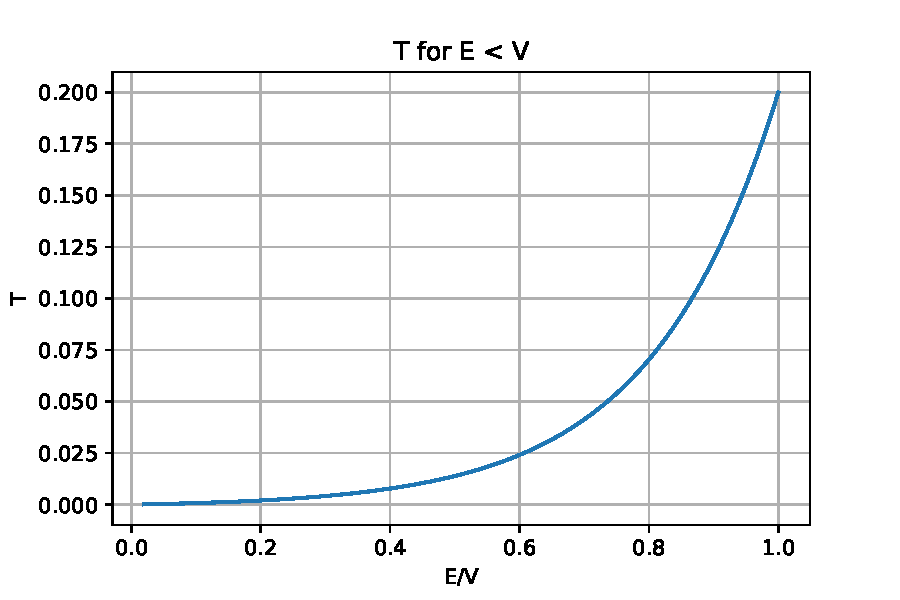
\includegraphics[scale=0.5]{images/TransmissionPropability2.pdf}
    \caption{Зависимость коэффициента подбарьерного перехода от энергии частицы}
    \label{fig:TransmissionPropability2}
\end{figure}
    
\end{frame}

\begin{frame}
\frametitle{Зависимость коэффициента надбарьерного перехода от энергии частицы}

\begin{figure}
    \centering
    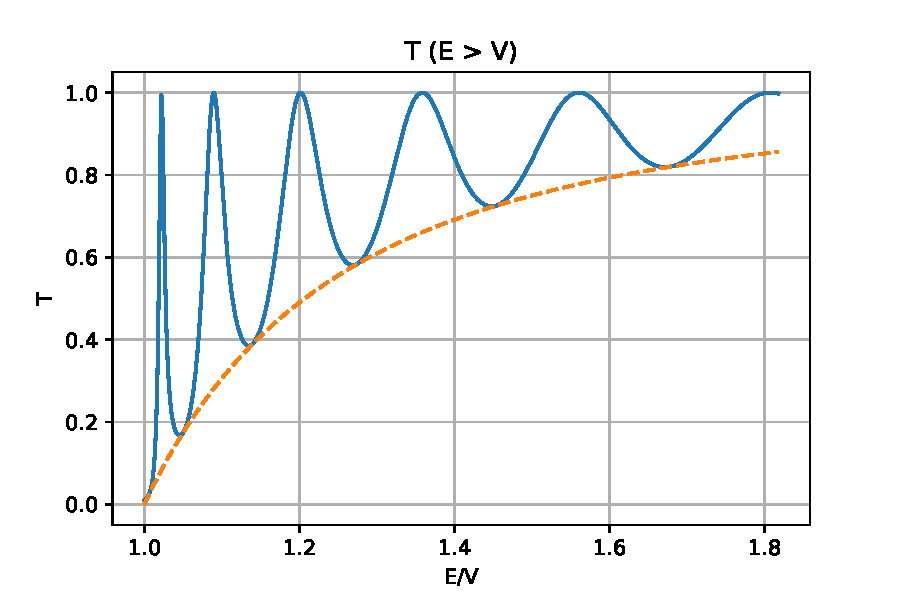
\includegraphics[scale=0.5]{images/TransmissionPropability1.pdf}
    \caption{Зависимость коэффициента надбарьерного перехода от энергии частицы}
    \label{fig:TransmissionPropability1}
\end{figure}
    
\end{frame}

\begin{frame}
\frametitle{Средний импульс и срядняя координата}

Зная значение волновой функции $\psi(x, t)$ в любой точке в любой момент времени, мы сможем расчитывать средние величины
по формулам

\begin{equation*}
    \langle x \rangle = \int \psi^* x \psi dx
\end{equation*}

\begin{equation*}
    \langle p \rangle = \int \psi^* \frac{\partial \psi}{\partial x} dx
\end{equation*}
    
\end{frame}

\begin{frame}
\frametitle{Действительная и мнимая части волновой функции}

\begin{figure}
    \centering
    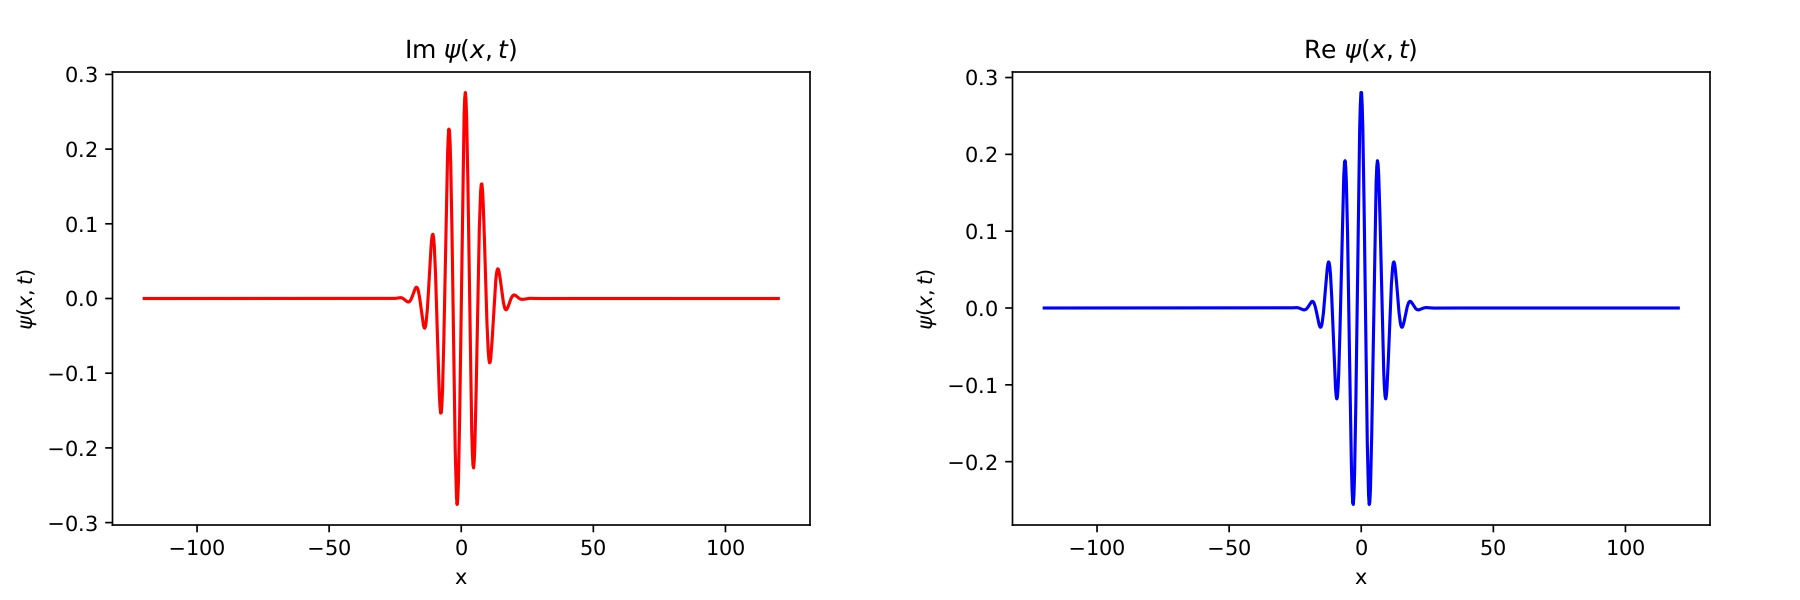
\includegraphics[scale=0.4]{images/PsiFunction.jpg}
    \caption{Действительная и мнимая части волновой функции}
    \label{fig:my_label}
\end{figure}
    
\end{frame}

\begin{frame}
\frametitle{Квадрат модуля волновой функции}

\begin{figure}
    \centering
    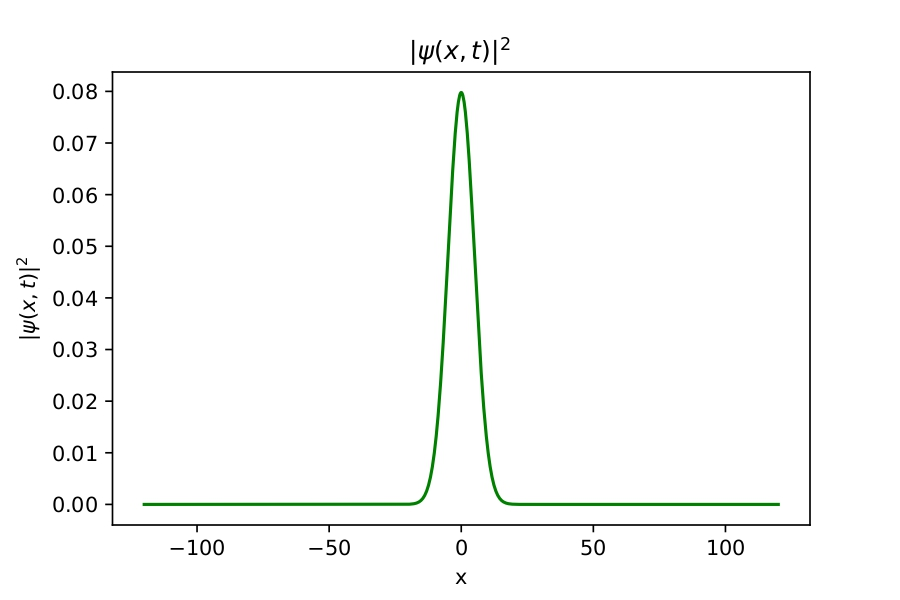
\includegraphics[scale=0.5]{images/PsiFunctionPropability.jpg}
    \caption{Квадрат модуля волновой функции}
    \label{fig:my_label}
\end{figure}
    
\end{frame}

\begin{frame}
\frametitle{Изменение волновой функции со временем}

\begin{figure}
    \centering
    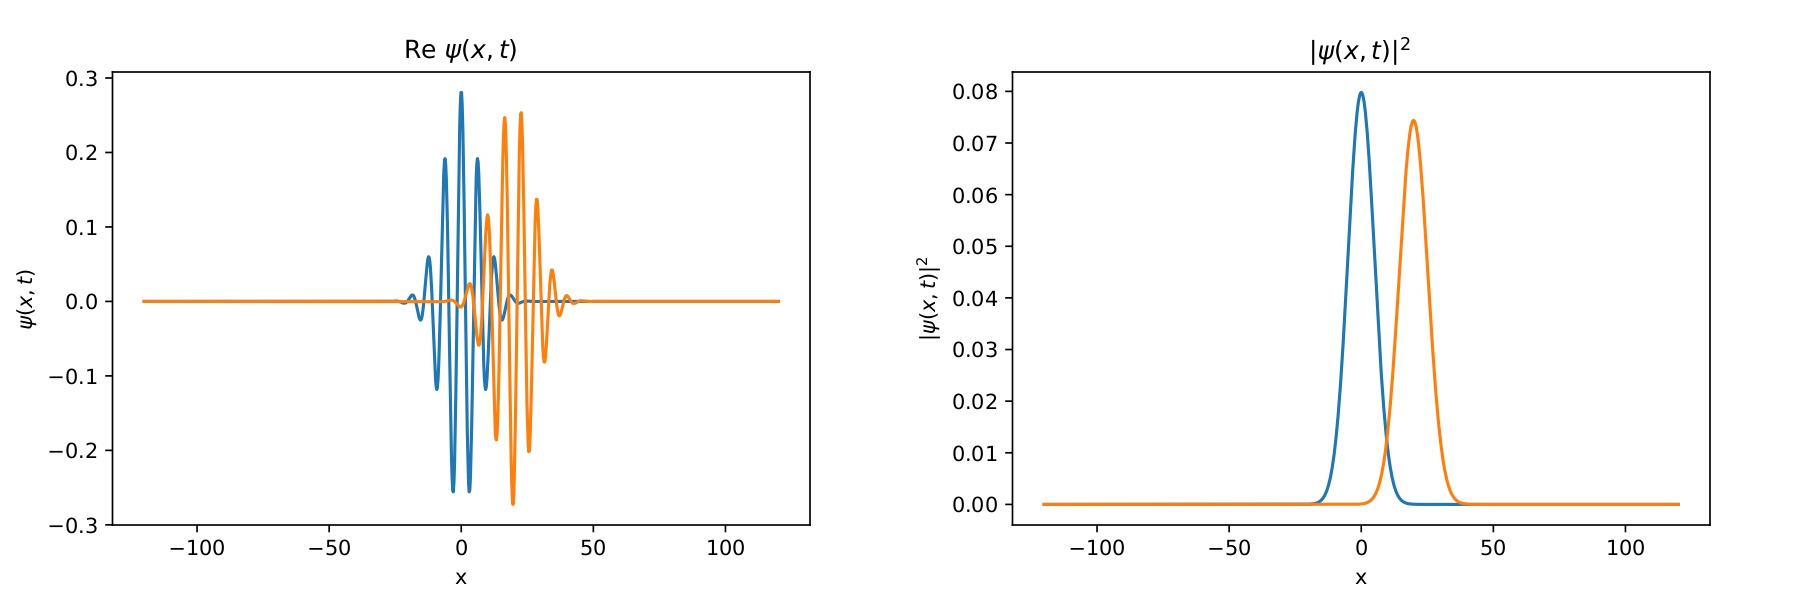
\includegraphics[scale=0.35]{images/PsiTimeEvol.jpg}
    \caption{Изменение волновой функции со временем}
    \label{fig:my_label}
\end{figure}
    
\end{frame}

\begin{frame}
\frametitle{Примеры моделей}

\begin{figure}
    \centering
    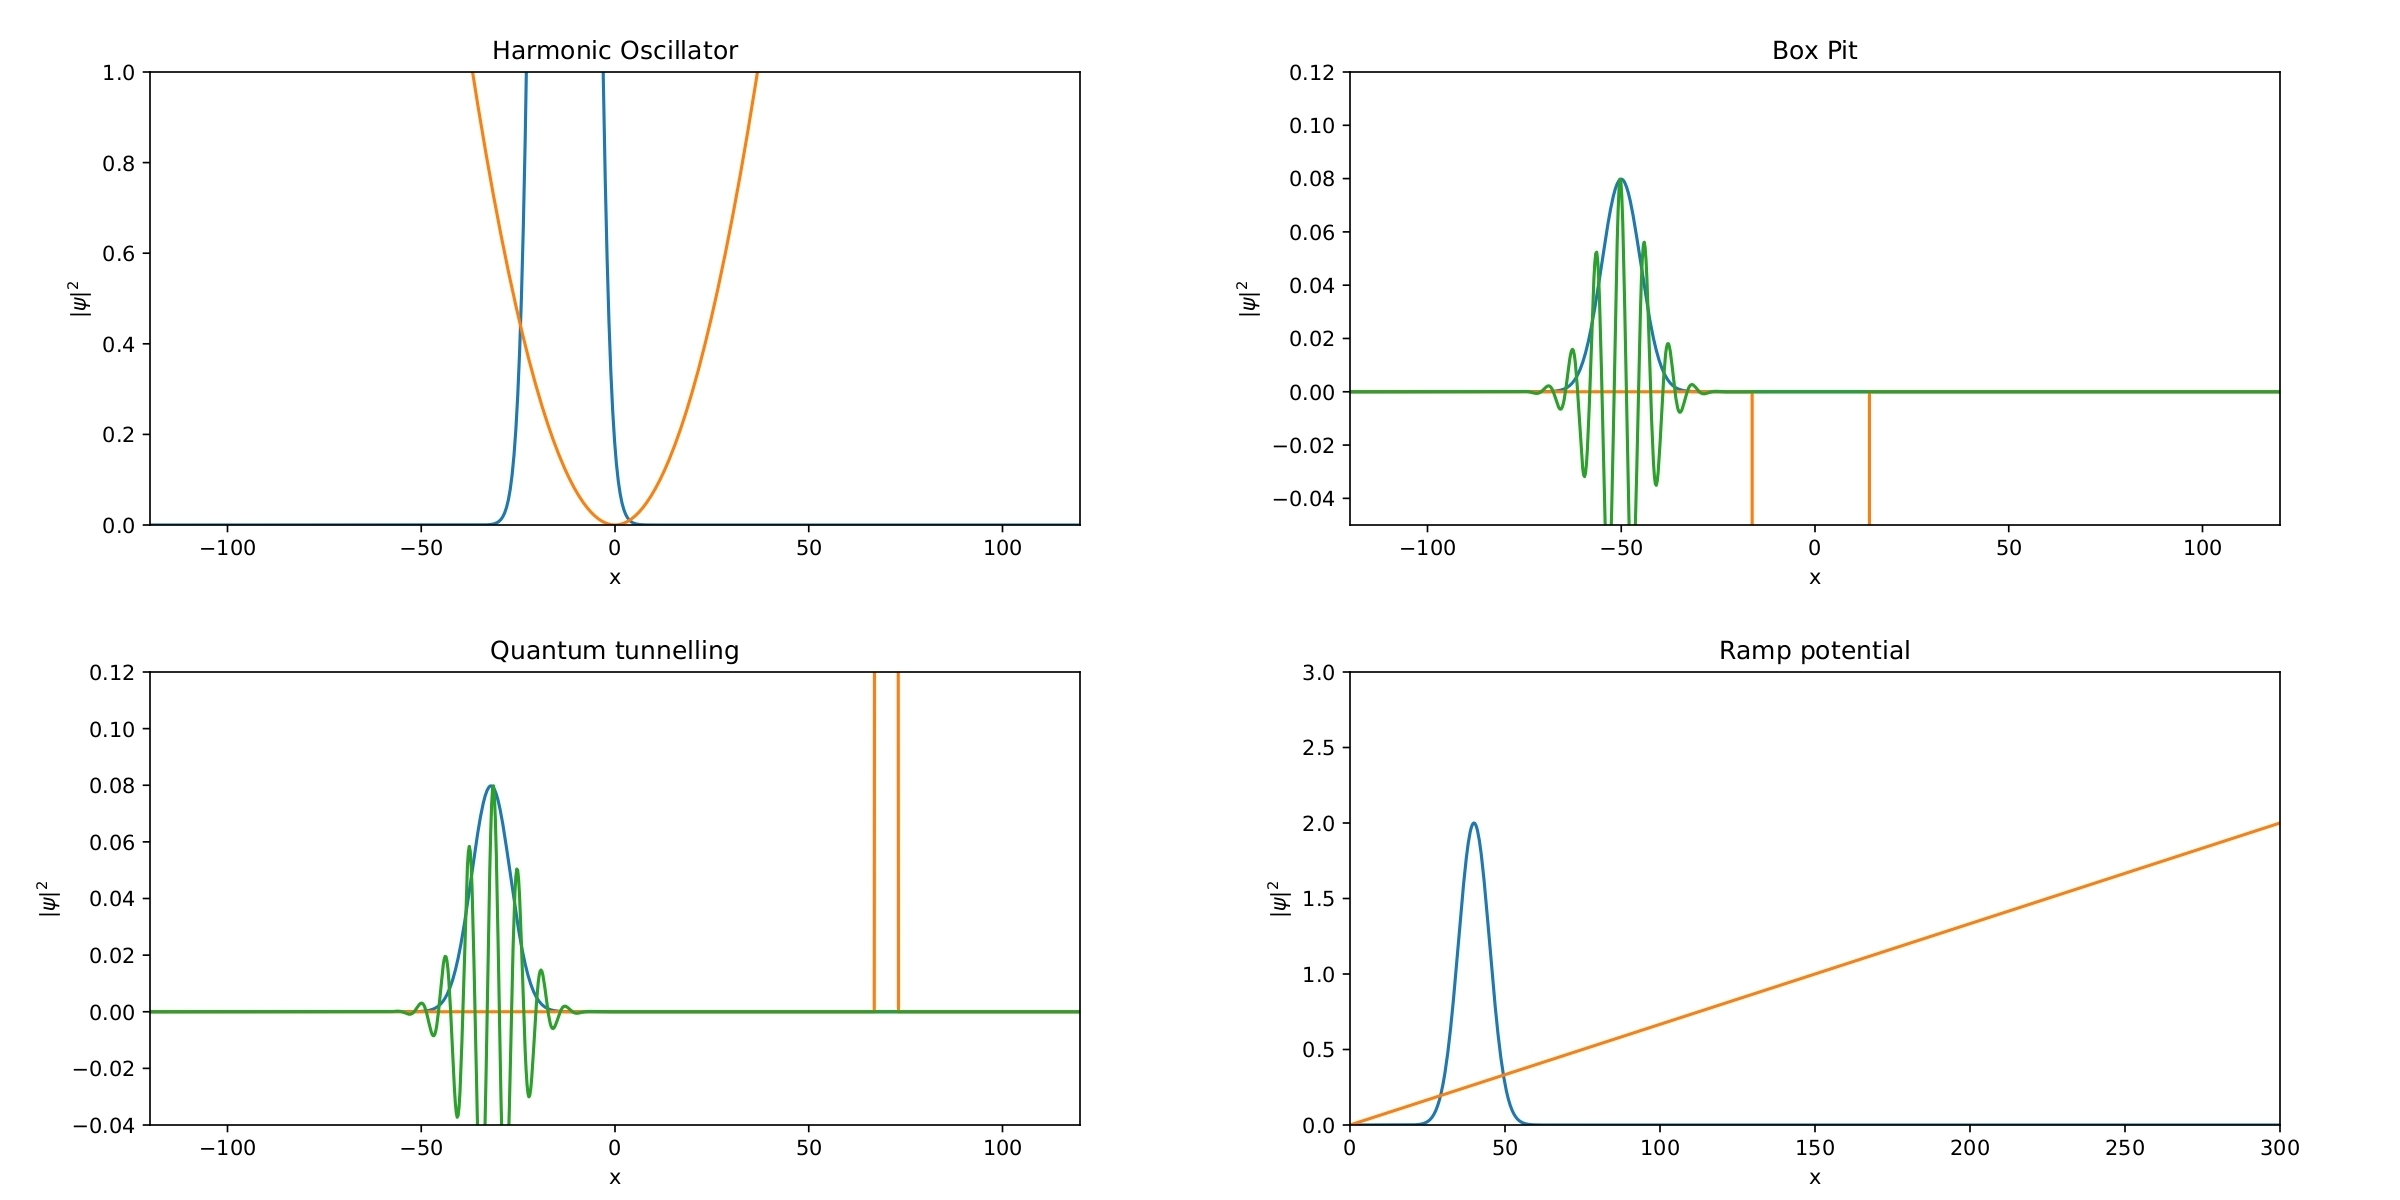
\includegraphics[scale=0.25]{images/merged.jpg}
    % \caption{Caption}
    % \label{fig:my_label}
\end{figure}
    
\end{frame}

\begin{frame}
\frametitle{Примеры моделей}

\begin{figure}
    \centering
    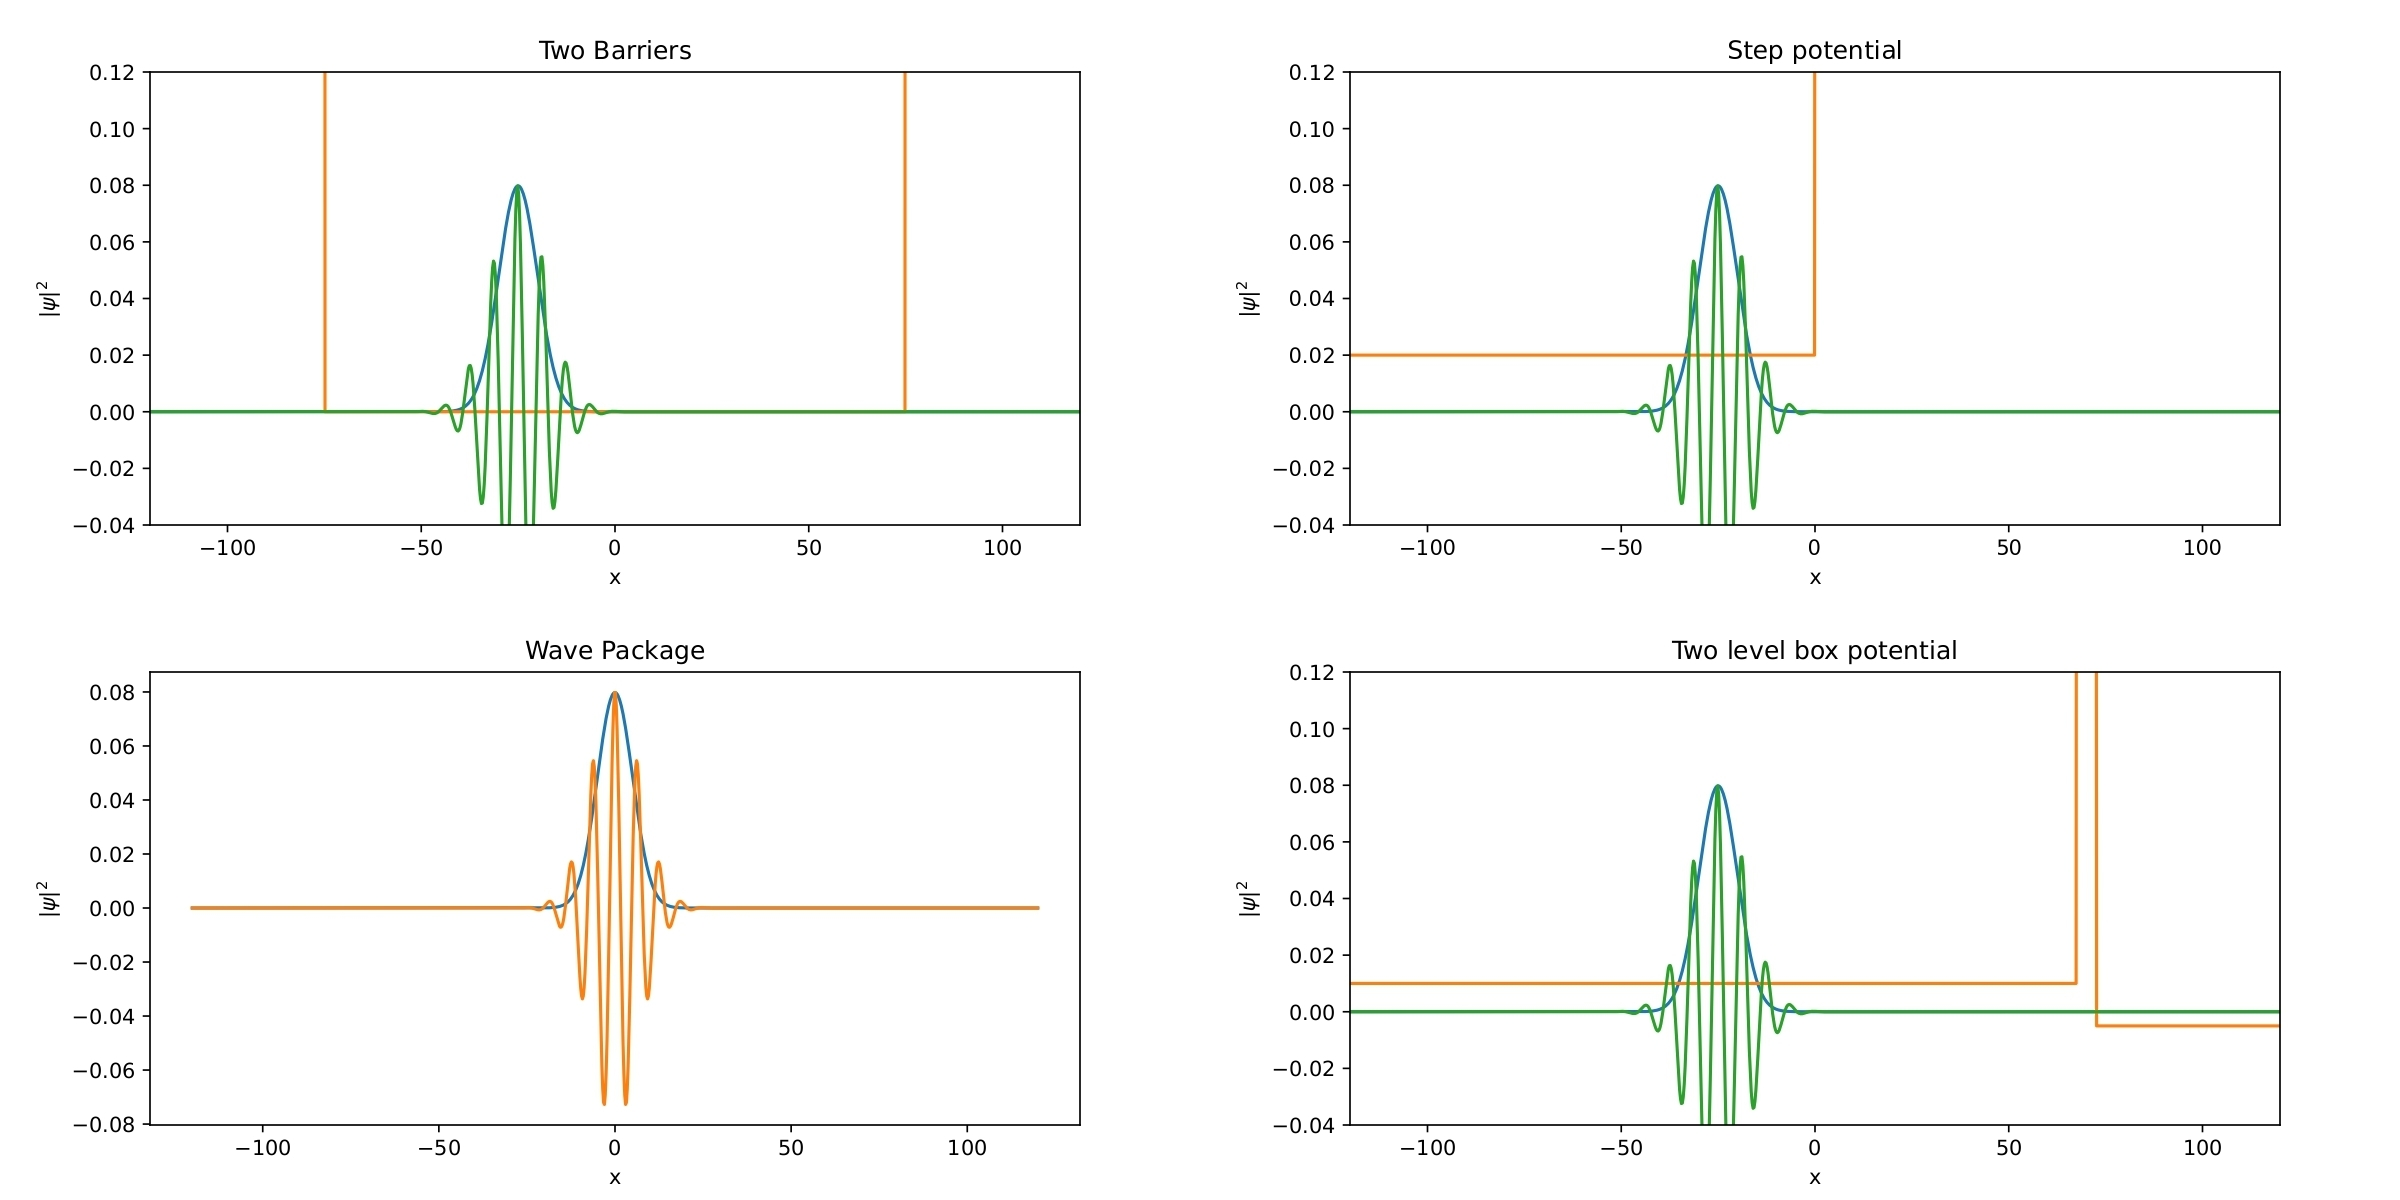
\includegraphics[scale=0.25]{images/merged2.jpg}
    % \caption{Caption}
    % \label{fig:my_label}
\end{figure}
    
\end{frame}

% \begin{frame}
% \frametitle{Волновая функция в отсутствии препятствий}

% \begin{figure}
%     \centering
%     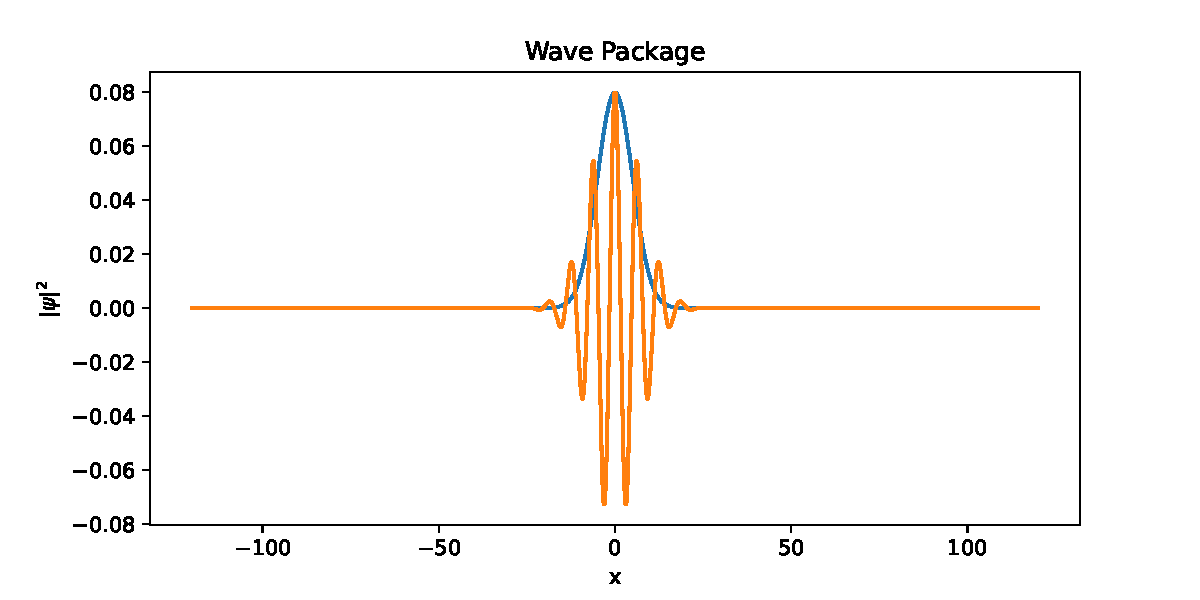
\includegraphics[scale=0.5]{images/WavePackage.pdf}
%     \caption{Волновая функция в отсутствии препятствий}
%     \label{fig:WavePackage}
% \end{figure}
  
% \end{frame}

% \begin{frame}
% \frametitle{Прямоугольная потенциальная яма}

% \begin{figure}
%     \centering
%     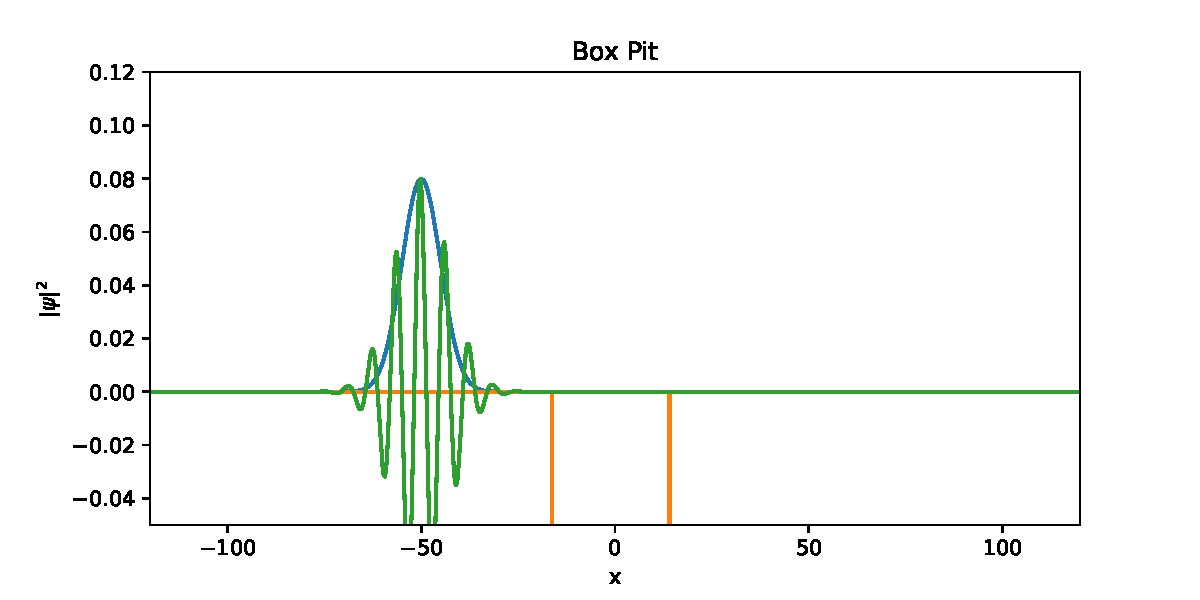
\includegraphics[scale=0.5]{images/BoxPit.pdf}
%     \caption{Прямоугольная потенциальная яма}
%     \label{fig:BoxPit}
% \end{figure}
  
% \end{frame}

% \begin{frame}
% \frametitle{Параболическая потенциальная яма}

% \begin{figure}
%     \centering
%     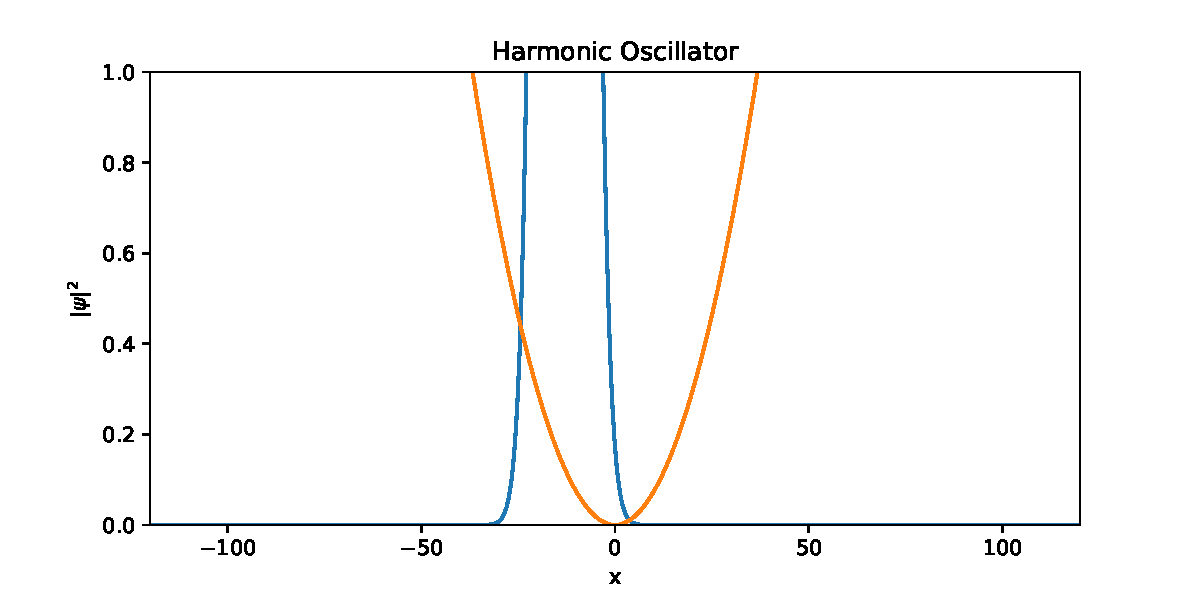
\includegraphics[scale=0.5]{images/HarmonicOscillator.pdf}
%     \caption{Параболическая потенциальная яма}
%     \label{fig:HarmonicOscillator}
% \end{figure}
  
% \end{frame}

% \begin{frame}
% \frametitle{Прямоугольный потенциальный барьер конечной ширины}

% \begin{figure}
%     \centering
%     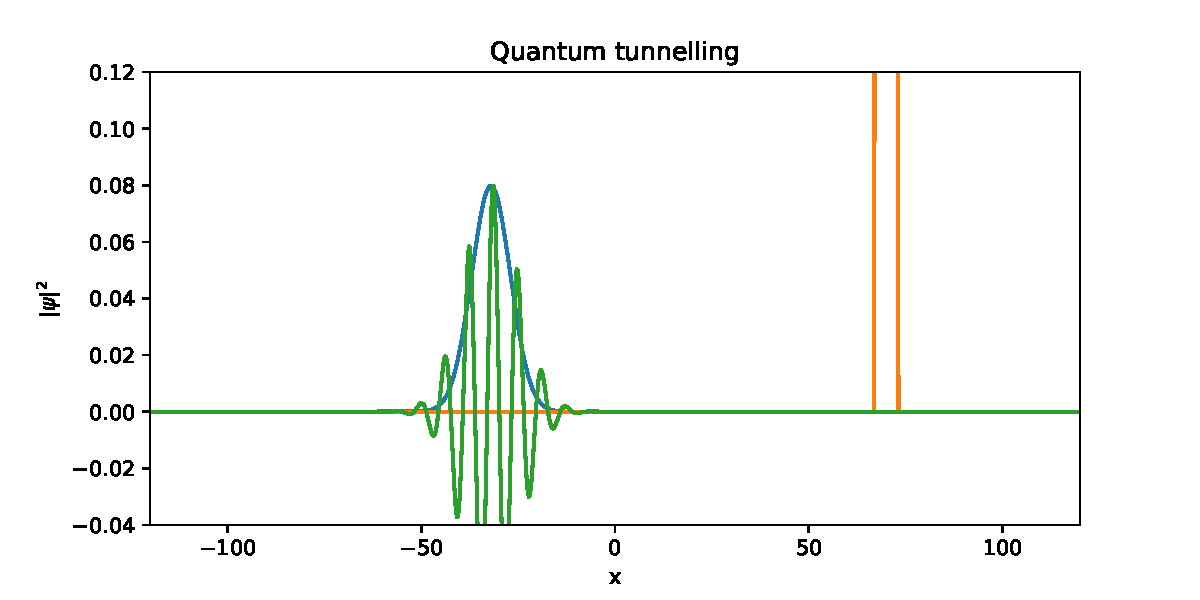
\includegraphics[scale=0.5]{images/QuantumTunnelling.pdf}
%     \caption{Прямоугольный потенциальный барьер конечной ширины}
%     \label{fig:QuantumTunnelling}
% \end{figure}

% \end{frame}

% \begin{frame}
% \frametitle{Равномерно возрастающий потенциал}

% \begin{figure}
%     \centering
%     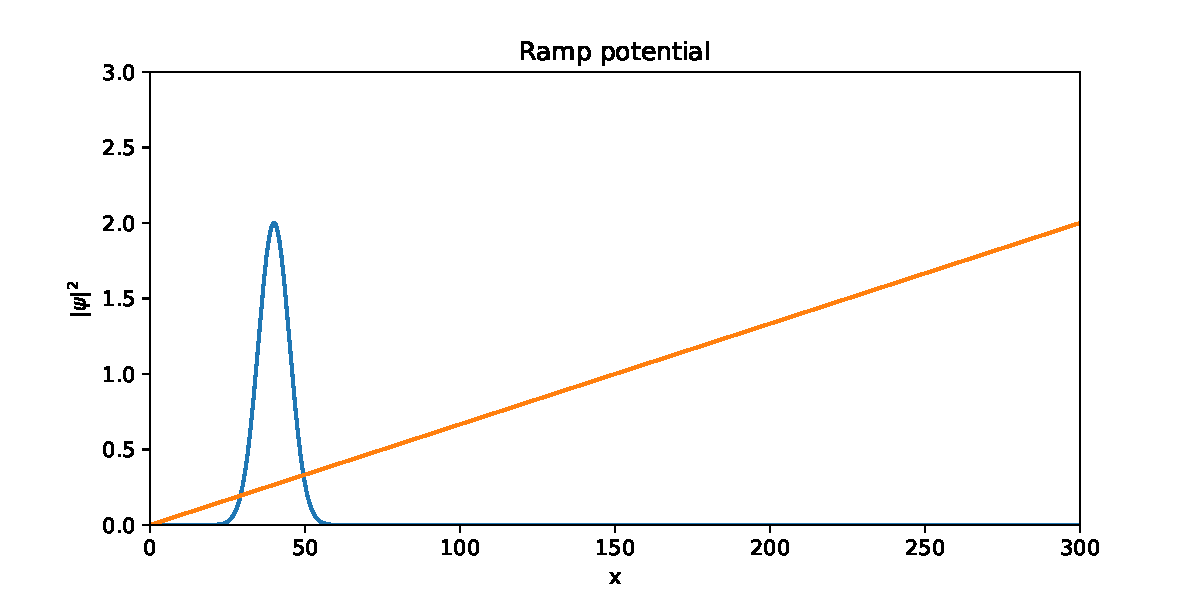
\includegraphics[scale=0.5]{images/RampPotential.pdf}
%     \caption{Равномерно возрастающий потенциал}
%     \label{fig:RampPotential}
% \end{figure}
    
% \end{frame}

% \begin{frame}
% \frametitle{Прямоугольный потенциальный барьер}

% \begin{figure}
%     \centering
%     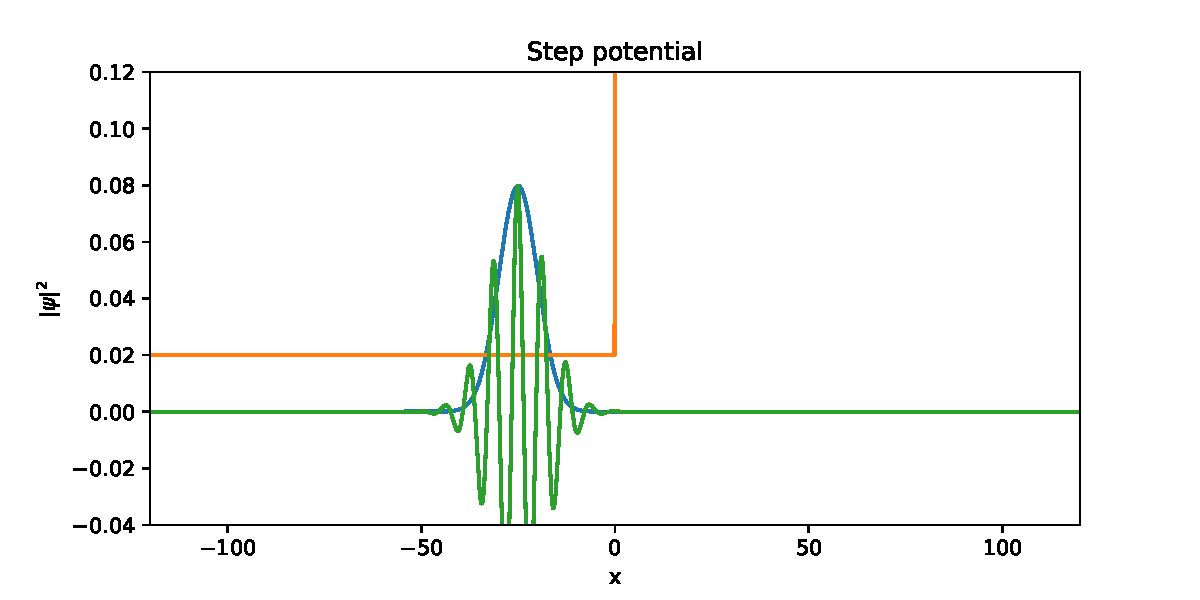
\includegraphics[scale=0.5]{images/StepPotential.pdf}
%     \caption{Прямоугольный потенциальный барьер}
%     \label{fig:StepPotential}
% \end{figure}

% \end{frame}

% \begin{frame}
% \frametitle{Бесконечно глубокая потенциальная яма}

% \begin{figure}
%     \centering
%     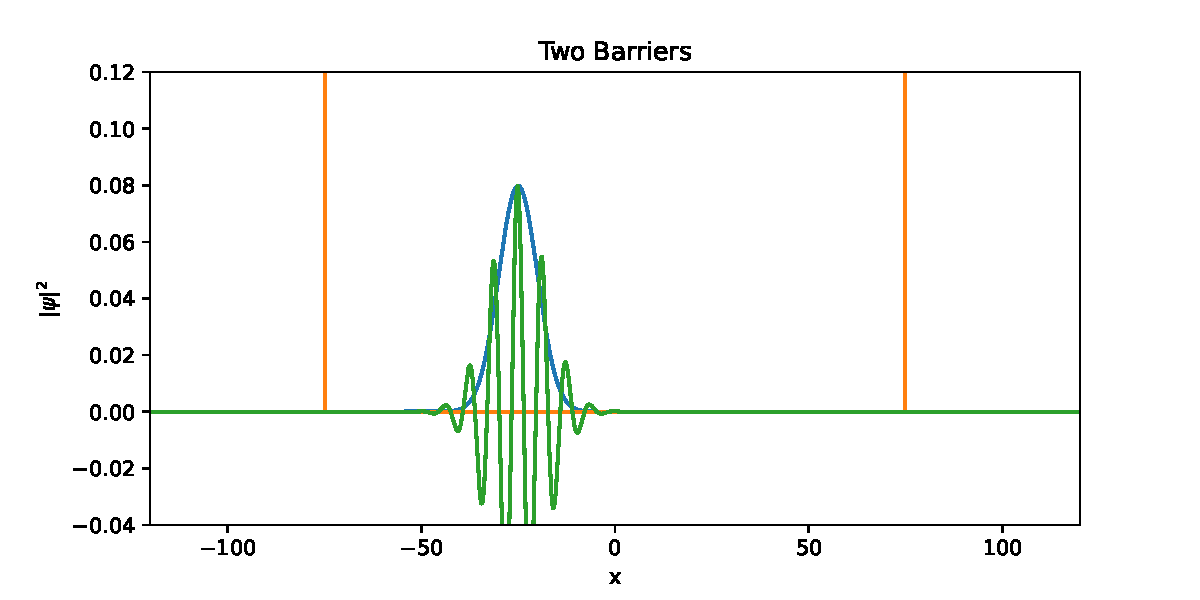
\includegraphics[scale=0.5]{images/TwoBarriers.pdf}
%     \caption{Бесконечно глубокая потенциальная яма}
%     \label{fig:TwoBarriers}
% \end{figure}
    
% \end{frame}

% \begin{frame}
% \frametitle{Общий случай прямоугольного потенциального барьера}

% \begin{figure}
%     \centering
%     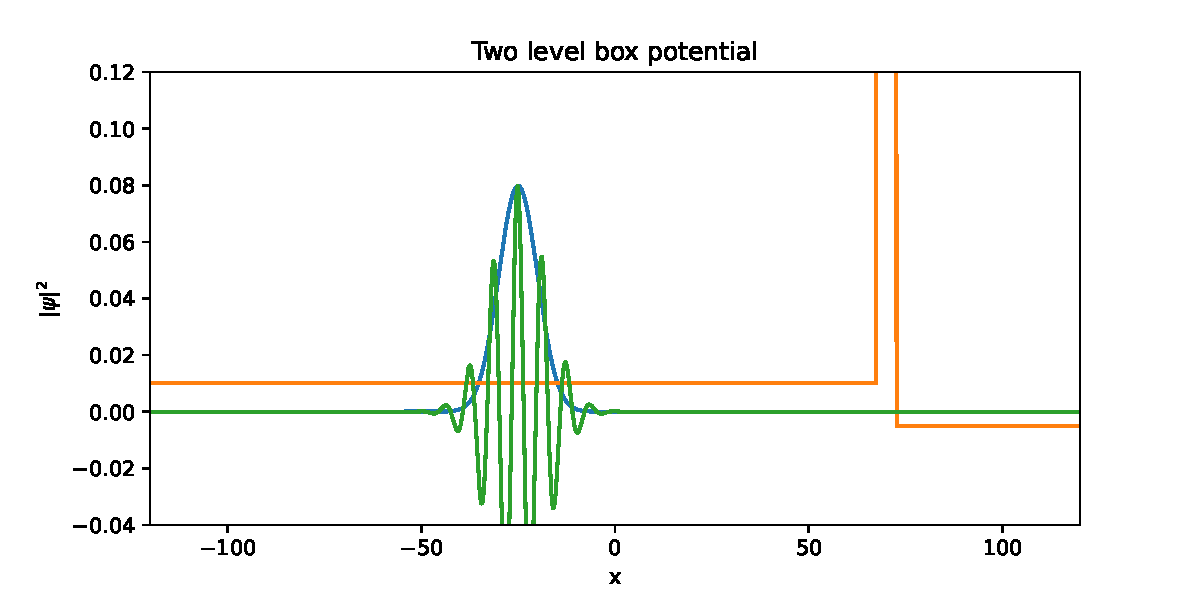
\includegraphics[scale=0.5]{images/TwoLevelBoxPotential.pdf}
%     \caption{Общий случай прямоугольного потенциального барьера}
%     \label{fig:TwoLevelBoxPotential}
% \end{figure}
    
% \end{frame}

\end{document}